\section{任意の winding を持つ分岐 block の actual annulus への挿入}
\label{ai:section}

本節では $t\ne0$ を固定する。第\ref{pw:m1}項の一次共役因子の模型から、
有限長の annulus 内へ縮小して入れられる compact block を切り出す。
全ての compact fibers を同時に移すので、focus germ だけの Darboux 同定ではない。
中心の disk まで同じ normal frame を延ばすことは要求しない。
この自由度を明示した上で、所定の K\"ahler form と一つの curve end に対する
actual な構成を与える。他の corner faces はこの段階では自由な境界である。

\subsection{Upper leg を切り、$x=0$ を避ける compact block}

標準 $\CC^3$ 上で、角は周期 $1$、$\rho_u=\pi|u|^2$ として
\[
 H_0=\rho_x+\rho_y,\qquad J_0=\rho_y-\rho_z,
 \qquad W_0=\bar x yz,\qquad Q_0=|W_0-c|^2,
 \qquad c>0
\]
と置く。$(h,j)$ の小さい compact rectangle $R$ を
$h>\max(0,j)$ の中に取り、全ての $(h,j)\in R$ で
$F_1(h,j)>2c$ とする。$R$ は $j=0$ を横切るものとする。
ここで $F_1$ は第\ref{pw:m1}項の radial maximum である。
Rectangle を十分小さくすれば、定数 $q_-,q_*,q_+$ を
\begin{equation}\label{ai:q-window}
 0<q_-<c^2<q_*<\min_R(F_1-c)^2
 \le\max_R(F_1-c)^2<q_+<\min_R(F_1+c)^2
\end{equation}
となるように選べる。$u=\rho_y$ とし、$u_1(h,j)$ を radial maximum point とする。
\begin{equation}\label{ai:K}
\begin{split}
 K={}&\{(H_0,J_0)\in R,\ q_*\le Q_0\le q_+\}\\
 &\ \cup\{(H_0,J_0)\in R,\ q_-\le Q_0\le q_*,\ u\le u_1(H_0,J_0)\}.
\end{split}
\end{equation}

\begin{proposition}\label{ai:compact-block}
$K$ は境界・角を持つ compact な領域で、$K\subset\{x\ne0\}$ である。
$Q_0<q_*$ では lower sheet の connected components のみを残し、
$Q_0\ge q_*$ では全 components を残している。
$Q_0=q_*$ における upper component の切断面は正則である。

$K$ 内の正則 connected fibers は $T^3$ である。
特異 fibers は、$j=0,Q_0=c^2$ の
$S^1\times$(once-pinched $T^2$) と、
$Q_0=(F_1(h,j)-c)^2$ の $T^2\times(S^1\vee S^1)$ である。
座標軸の elliptic--elliptic points、$Q_0=0$ の minima、還元された maximum は $K$ に入らない。
Saddle の近くの connected-fiber quotient は $R\times Y$ 型である。
ここで saturated とは、元の map の fibers の connected components に関する意味である。
\end{proposition}

\begin{proof}
$(H_0,J_0,Q_0)$ は proper なので、式\eqref{ai:K}の閉集合は compact である。
さらに $H_0=h$, $J_0=j$ なら
\[
 \rho_x+\rho_y+\rho_z=h+\rho_z\le 2h+|j|
\]
という直接の bound もある。
$q\le q_*$ では $c+\sqrt q<F_1(h,j)$ なので、
circle $|W_0-c|^2=q$ 全体が radial double disk の内部に入る。
従って二つの sheets は分離し、$u<u_1$ の方が lower component である。
$u=u_1$ では $Q_0\ge(F_1-c)^2>q_*$ だから、
式\eqref{ai:K}の sheet 条件が新しい境界を作ることはない。
Upper component の $q=q_*$ は、saddle value と異なる正則な切断面である。

$x=0$ なら $W_0=0$、従って $Q_0=c^2<q_*$ であり、
$u=h>u_1$ なので $K$ から除外される。
Compactness から $|x|$ は $K$ 上で正の下界を持つ。
他の二つの非零座標軸も $x=0$ に含まれるので除かれる。
残る rank drops は第\ref{pw:m1}項の分類と式\eqref{ai:q-window}により、
記載した focus と smooth saddle に限られる。
$j=0,Q_0=c^2$ では upper regular component は除かれ、lower compact focus component の全体が残る。
Saddle value は $q_*$ より大きいので、saddle fiber の全体も残る。
第\ref{pw:m1}項の connected-level quotient と principal $T^2$-bundle の記述を適用する。
Boundary の transversality も確認できる。$j=0$ は $R$ の内部にあり、
focus axis 上の $H_0$ は regular である。残る $(H_0,J_0)$ の rectangle faces では
必要な moment differentials は独立であり、全ての $Q_0$ 切断値はその faces 上でも regular である。
従って各 faces は通常の角として交わり、$u=u_1$ による隠れた seam は生じない。
\end{proof}


\begin{figure}[tbp]
\centering
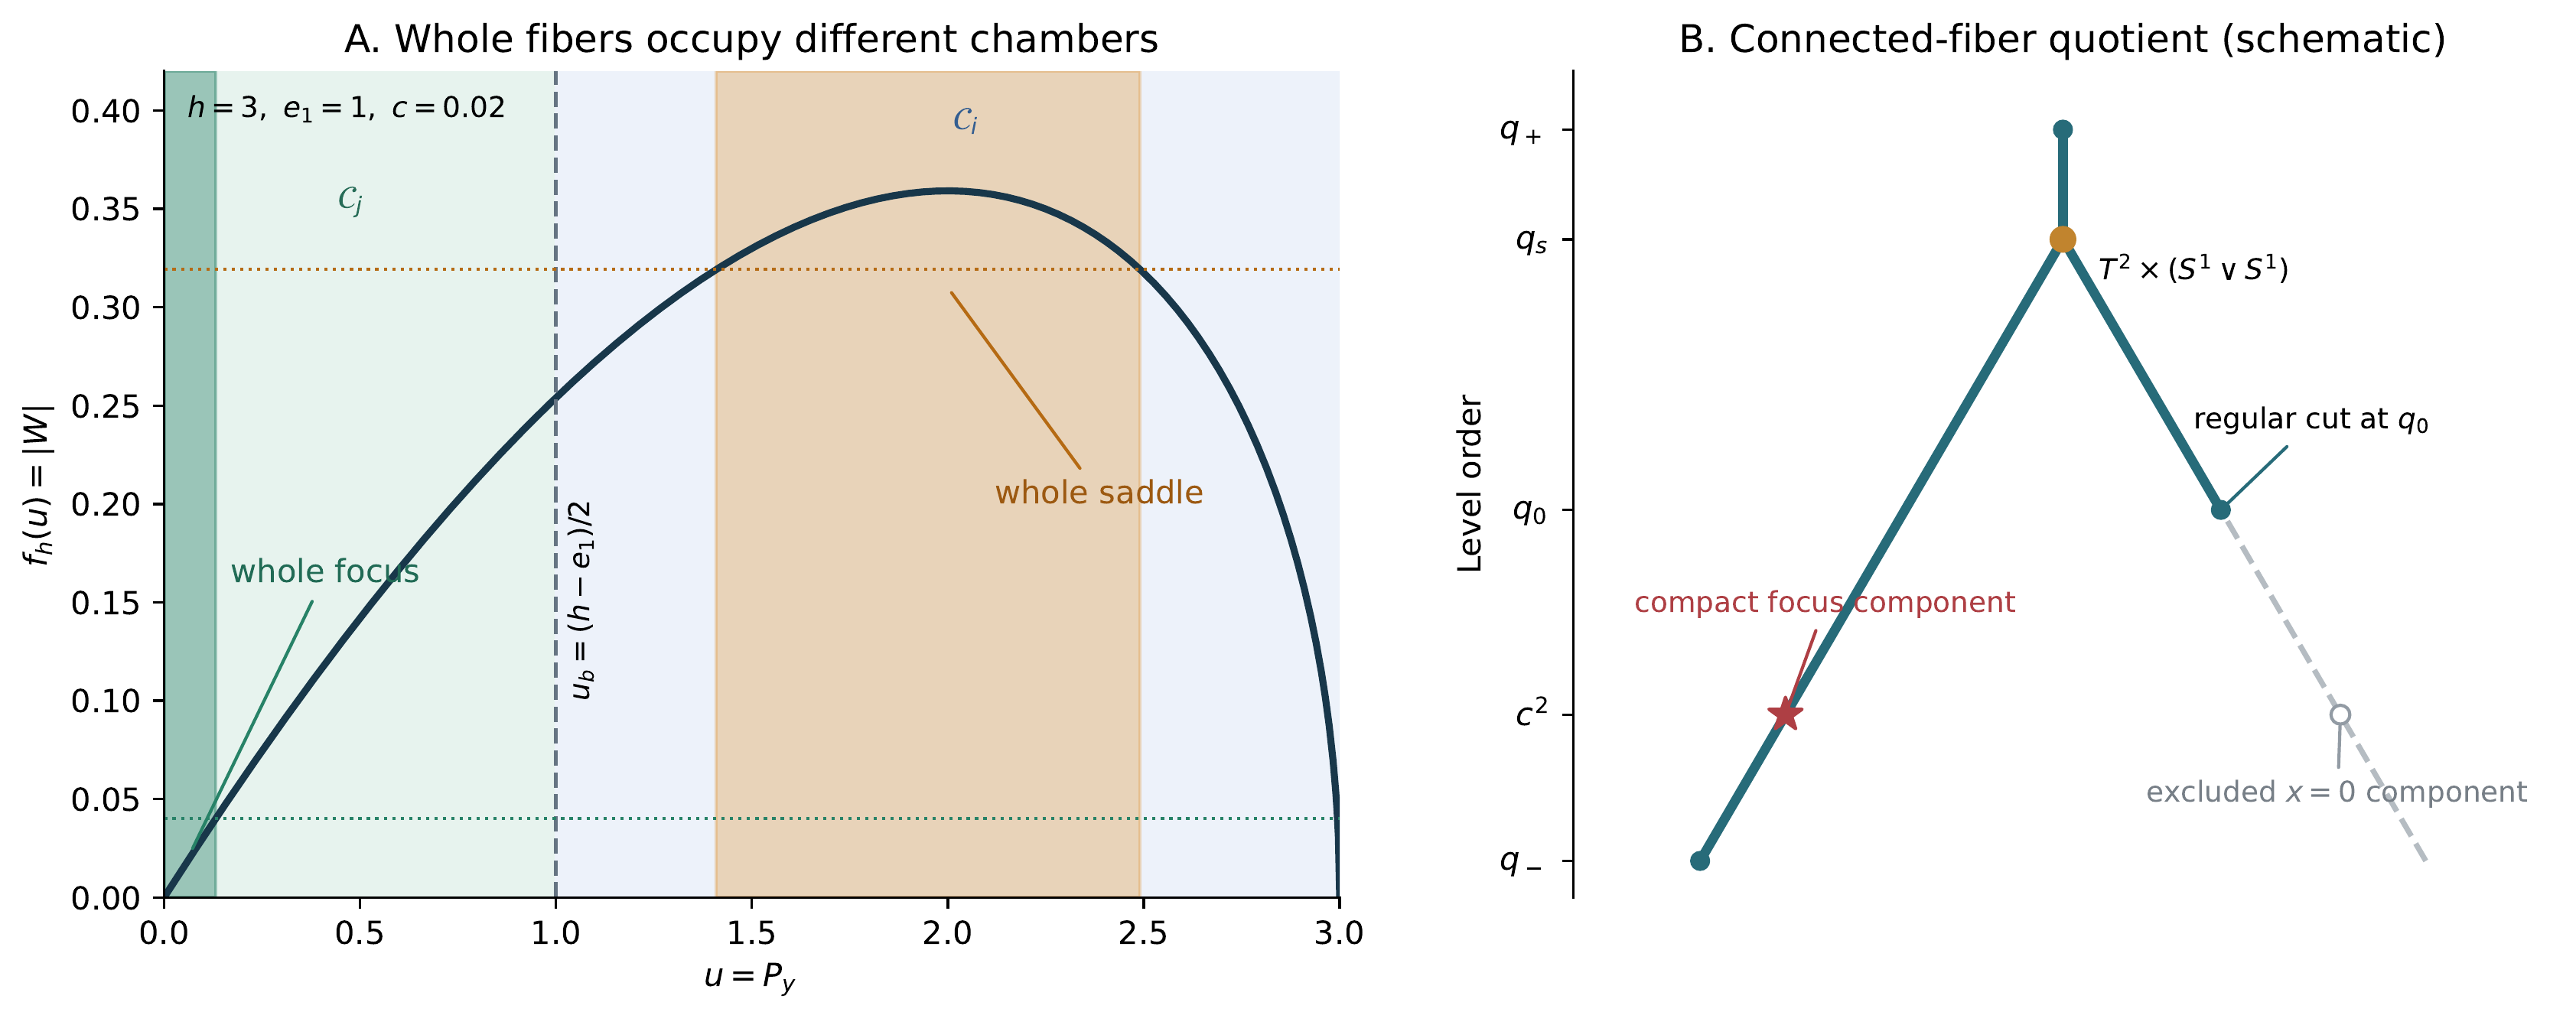
\includegraphics[width=\textwidth]{positive_transport_geometry.png}
\caption{左は chosen graph form における whole focus と whole saddle の chamber 分離。
右は annular insertion に用いる connected-fiber quotient の模式的な断面で、縦方向は level の順序だけを表す。
Upper leg の $q_0>c^2$ での切断により $x=0$ を含む成分を除き、lower focus と true saddle を保持する。
図の $q_0$ は本文の $q_*$ に対応する。}
\label{ai:figure}
\end{figure}

\subsection{明示的な annular embedding と primitive の定数項}

標準 normal tube を
\[
 \mathcal T=(I_-,I_+)\times S^1_\theta\times\CC^2_{Y,Z},\qquad
 \lambda_{\mathcal T}=I\,d\theta+\rho_Yd\theta_Y+\rho_Zd\theta_Z,
 \qquad\Omega_{\mathcal T}=d\lambda_{\mathcal T}
\]
とする。$b\in(I_-,I_+)$、$k\in\ZZ$ を任意に固定する。
$s>0$ に対し、$\{x\ne0\}$ の上で
\begin{equation}\label{ai:embedding}
 \theta=\frac{\arg x}{2\pi},\qquad
 Y=\sqrt{s}\,e^{2\pi i(k-1)\theta}y,\qquad Z=\sqrt{s}\,z,
 \qquad I=b+s\bigl(\rho_x-(k-1)\rho_y\bigr)
\end{equation}
と定める。

\begin{theorem}\label{ai:insertion}
任意の $k\in\ZZ$ と任意に小さい normal radius に対し、
$s>0$ を十分小さく取れば式\eqref{ai:embedding}は $K$ の開近傍を
$\mathcal T$ のその radius 内へ埋め込む。
この写像 $\iota_s$ は
\begin{equation}\label{ai:primitive}
 \iota_s^*\lambda_{\mathcal T}=s\lambda_0+b\,d\theta,
 \qquad \iota_s^*\Omega_{\mathcal T}=s\omega_0
\end{equation}
を満たす。従って $K$ の compact Lagrangian fibers、focus fibers、saddle fibers は
全て同時に actual な Lagrangian fibers へ移る。

像上の commuting integrals は
\begin{align}
 H&=I-b+k\rho_Y,& J&=\rho_Y-\rho_Z,\label{ai:integrals}\\
 W&=\sqrt{\frac{I-b+(k-1)\rho_Y}{\pi}}\,
       e^{-2\pi ik\theta}YZ,& Q&=|W-s^{3/2}c|^2.\label{ai:W}
\end{align}
Pullbacks はそれぞれ $sH_0,sJ_0,s^{3/2}W_0,s^3Q_0$ である。
Square root の中身は像の近傍で正である。
Focus axis における mixed coefficient の clockwise winding は、tube の frame に関して $k$ である。
\end{theorem}

\begin{proof}
式\eqref{ai:embedding}より
\[
 \iota_s^*(\rho_Yd\theta_Y)
 =s\rho_y\bigl(d\theta_y+(k-1)d\theta\bigr),
 \qquad \iota_s^*(\rho_Zd\theta_Z)=s\rho_zd\theta_z.
\]
$I\,d\theta$ と加えると、$\rho_y d\theta$ の補正が厳密に消え、
式\eqref{ai:primitive}を得る。Inverse は
\[
 x=\sqrt{\frac{I-b+(k-1)\rho_Y}{\pi s}}e^{2\pi i\theta},\quad
 y=s^{-1/2}e^{-2\pi i(k-1)\theta}Y,\quad z=s^{-1/2}Z
\]
である。$K$ 上では $\rho_x$ が正の下界を持つので、正の square root の領域に
少し大きい開近傍を取れ、そこで滑らかな embedding になる。
$K$ 上の $\rho_x,\rho_y,\rho_z$ は有界であるから、$I-b=O(s)$、
$|Y|,|Z|=O(\sqrt s)$ が一様に成り立つ。
これにより任意に小さい tube へ、全 compact fibers を保って入れられる。

式\eqref{ai:integrals}--\eqref{ai:W}の pullback は直接代入で分かる。
定数倍の symplectic form に対しても Poisson commutativity と Lagrangian 性は保たれる。
Zero section 上の focus locus では $I-b>0$ であり、
$Q$ の mixed quadratic coefficient は、正の実数倍と一定の非零実数を除けば
$e^{-2\pi ik\theta}$ である。Clockwise boundary での winding は $k$ となる。
\end{proof}

\begin{remark}[保持する marked periods]
任意の closed cycle $\gamma\subset K$ に対して、厳密に
\begin{equation}\label{ai:period}
 \int_{\iota_s\gamma}\lambda_{\mathcal T}
 =s\int_\gamma\lambda_0+b\,\deg(\theta|_\gamma)
\end{equation}
である。$b\,d\theta$ を exact term として捨ててはいけない。
Transverse cycle の $\theta$-degree が零なら、その action は $s$ 倍される。
Longitudinal circle の action には $b$ が加わる。
Hamiltonian $H$ の flow は周期 $1$ だが、primitive との contraction は
$\lambda_{\mathcal T}(X_H)=H+b$ である。
ここでは $\iota_{X_H}\Omega=-dH$ の規約を用いている。
\end{remark}

\begin{remark}[Disk-extension と semistable phase]
本定理の winding $k$ は、選んだ tube frame に関する値である。
Tube frame を actual semistable determinant frame の Hermitian 規格化から選べば、
これがそのまま central-frame winding になる。
第\ref{pw:semistable-phase}項の original-coordinate comparison における $+1$ を
さらに加えることはしない。本定理では式\eqref{ai:embedding}により新しい normal first jet を選んでいる。
特に original-coordinate identity $y=tY/x$ を保つ symplectic comparison を構成したわけではない。
Frame と action は有限 annulus 上では滑らかだが、同じ選択が deleted disk へ延びるとは限らない。
この点が第\ref{cw:section}節の disk-extending rigidity との両立理由である。
\end{remark}

\subsection{所定の K\"ahler form に対する actual tube}

\begin{lemma}[First jet を指定した annular neighborhood]
\label{ai:actual-tube}
$(X,\omega)$ を symplectic 六次元多様体、$C\subset X$ を symplectic surface、
$A\subset C$ を compact annulus とする。
$\omega|_A=dI\wedge d\theta$ と area coordinates を取り、
symplectic normal bundle の unitary frame を $A$ 上で選ぶ。
このとき、十分小さい標準 tube $\mathcal T$ から $X$ への symplectic embedding $\Psi$ があり、
zero section は $A$ へ恒等的に写り、normal first jet は指定した frame と一致する。
既に一つの小さい collar 上でこのような embedding が指定されていれば、
その collar を縮めた上で embedding 全体を厳密に保つ relative 版も成立する。
\end{lemma}

\begin{proof}
Symplectic normal を $TC^\omega$ とし、指定 frame と base の恒等写像から
zero section 上の symplectic linear isomorphism を作る。
これを smooth tubular embedding $F$ に延長する。
$F^*\omega$ と $\Omega_{\mathcal T}$ は zero section 上で full bilinear forms として一致する。
差を $\Delta$ と書く。Normal radial homotopy によって
$\Delta=d\alpha$、$\alpha=O(|v|^2)$ を得る。
十分小さい tube では直線経路 $\Omega_{\mathcal T}+u\Delta$ が symplectic であり、
$\iota_{V_u}(\Omega_{\mathcal T}+u\Delta)=-\alpha$ の Moser field は $V_u=O(|v|^2)$ となる。
従ってその flow は zero section と first jet を固定する。
Compactness により共通の小さい tube 上で time $1$ まで定義され、所要の $\Psi$ を得る。
Prescribed collar で $F$ を既存の embedding と一致させれば $\Delta=0$、
radial primitive も零となるため、Moser flow はそこで恒等である。
これは symplectic neighborhood theorem の relative Moser 証明である
\cite[\S7.3, Theorem 7.4]{cds-local}。
\end{proof}

K\"ahler 多様体内の complex curve collar を扱う場合にも、
complex normal frame が所定の K\"ahler metric に関して直交するとは限らない。
ただし一つの complex normal line を選び、それと Hermitian complement を使うことはできる。
Gram--Schmidt の diagonal coefficients を正に取ると、complex determinant は正実数倍なので、
元の determinant frame に対する winding は変わらない。
この操作は一方の line を保持するが、指定された二つの非直交な normal lines の両方を保持しない。
その両方を固定することは、本節の結論に含めない。

\begin{corollary}[Actual K\"ahler annulus 内の branched block]
\label{ai:actual-insertion}
補題\ref{ai:actual-tube}の任意の actual tube に対し、任意の整数 $k$ の winding を持つ
compact block $\Psi(\iota_s(K))$ が、十分小さい $s>0$ について存在する。
その全 fibers と singularity types は命題\ref{ai:compact-block}の通りであり、
元の $\omega$ に関して Lagrangian である。
Actual form が coordinate torus rotations に不変であることは必要ない。
Hamiltonian actions も $\Psi\circ\iota_s$ により同時に移送する。
\end{corollary}

Actual tube 上に primitive $\lambda_X$ が既に指定されている場合にも、
その $A$ 上の circle period を用いて $I$ の additive constant を決めれば、
$\Psi^*\lambda_X-\lambda_{\mathcal T}$ の $H^1(\mathcal T;\RR)$ class は零となる。
従ってこの差は exact であり、式\eqref{ai:period}は同じ marked cycles に対してそのまま成り立つ。
Additive constant と配置する $b$ は、primitive の period データとして保持する。
所定の global primitive がなくても、$H^2(\mathcal T;\RR)=0$ により local primitive は選べる。

\subsection{一つの curve end との whole-fiber 一致}

式\eqref{ai:embedding}の像上で
\[
 \widehat H=H+b=I+k\rho_Y,\qquad
 U=e^{-2\pi ik\theta}Y,\qquad V=Z
\]
と置くと、厳密に
\begin{equation}\label{ai:end-coordinates}
 \lambda_{\mathcal T}=\widehat H\,d\theta+\rho_Ud\theta_U+\rho_Vd\theta_V,
 \quad J=\rho_U-\rho_V,
 \quad W=\sqrt{\frac{\widehat H-b-\rho_U}{\pi}}\,UV
\end{equation}
となる。すなわち、一次共役因子の decreasing radial family が
$a=\widehat H-b$ としてそのまま現れる。
この式は単なる quadratic approximation ではなく、compact lower component 全体での恒等式である。

\begin{theorem}[一つの actual positive-winding end の接着]
\label{ai:one-end}
$\bar C\subset(X,\omega)$ を compact symplectic surface with boundary とし、
boundary components の数を $n\ge2$ とする。
一つの boundary collar に補題\ref{ai:actual-tube}の tube を選ぶ。
他の端の fibration と normal frames を自由に選んでよいとする。
このとき、任意の $k\in\ZZ$ に対し、十分小さい annular branched block と
curve block を actual $\omega$ の上で接ぐことができる。
接着部分は lower compact focus component の saturated collar であり、
両側の actual fibers、period-one circle actions、marked primitive periods は厳密に一致する。
Corner の内部には whole $T^2\times(S^1\vee S^1)$ saddle fiber が残る。
他の artificial boundary faces の消失は主張しない。
\end{theorem}

\begin{proof}
第\ref{pw:m1}項の $F_1>2c$ の範囲で、$j=0,q=c^2$ の lower component を含む
小さい compact $(j,q)$-window を取る。Lower root と upper root の間には一様な gap がある。
従って window を縮めれば、選んだ $H$-interval 上で全 lower fibers を一つの normal tube に入れられる。
具体的な cutoff 不等式は補題\ref{pe:uniform}による。
式\eqref{ai:end-coordinates}をそのまま curve block の prescribed collar germ とする。

Normal first jet は、tube frame に対して $U$-direction を $e^{2\pi ik\theta}$ 倍する。
この first jet は annulus 上では unitary である。Disk への延長は要求しない。
$n\ge2$ の surface では、一つの boundary circle に指定した $S^1$-valued frame の degree を
別の自由な boundary で相殺できる。従って二つの individual frames と tensor frame は
$\bar C$ 上へ延長できる。
これは $H^2(\bar C;\ZZ)=0$ と、一つの boundary への
$H^1(\bar C;\ZZ)\to H^1(S^1;\ZZ)$ の全射性からも従う。

この延長を用いて dual connections を選び、指定 collar 上では connection forms を厳密に零とする。
Curve の Morse function と正の radial parameter $a$ は、指定 collar で
$a=\widehat H-b$ となるように選び、critical levels の近くでは必要な一定値にする。
定理\ref{pe:two-end}の一端だけを指定する構成により compact curve fibers を得る。
Normal radii は共通に十分小さく取る。

Curve model の embedding は、指定 collar 上では既に得た actual embedding と一致させる。
その first jet は上で global normal bundle へ延長されている。
Tubular embedding をこの germ に合わせて延ばし、補題\ref{ai:actual-tube}の relative Moser を使うと、
collar 全体を固定して actual $\omega$ へ移せる。
したがって germ だけでなく、その domain に含まれる compact focus fiber 全体と近傍 fibers が一致する。

Primitive は collar 上で式\eqref{ai:end-coordinates}を使用する。
Base primitive のこの一つの boundary period は、他の自由な boundary periods を調整して延長できる。
よって longitudinal shift $b$ を含む marked periods が一致する。
ここで relative embedding を固定する collar は、lower fibers だけでなく
$\iota_s(K)$ 全体を式\eqref{ai:end-coordinates}で表示できる normal neighborhood を含むものとする。
必要なら zero-section collar を少し延長してから切断位置を選ぶ。
$K$ はこの共通座標で $\widehat H\in b+s\,\operatorname{pr}_h R$ に射影し、
normal radii は一様に $O(\sqrt s)$ なので、十分小さい $s$ に対してこの選択ができる。
共通 collar 上では、curve block の $(J,Q)$-window と lower-root cutoff によって
交わりを lower connected components に限定する。
Collar 外も同じ global normal embedding を用いるので、その単射性により余分な交わりは生じない。
指定 collar の両側を切って接げば、共通の actual fibers を持つ一つの compact assembly となる。
\end{proof}

\subsection{半安定超曲面における適用範囲}

\begin{proposition}[二つの normal lines への winding の配分]
\label{ai:distributed}
整数 $a,d$ に対し、式\eqref{ai:embedding}を
\begin{equation}\label{ai:distributed-map}
\begin{aligned}
 Y&=\sqrt{s}\,e^{2\pi i(a-1)\theta}y,&
 Z&=\sqrt{s}\,e^{2\pi id\theta}z,\\
 I&=b+s\bigl(\rho_x-(a-1)\rho_y-d\rho_z\bigr)
\end{aligned}
\end{equation}
で置き換えても、式\eqref{ai:primitive}と全 compact fibers の挿入が成り立つ。
その winding は $k=a+d$ であり、像上では
\begin{align}
 H&=I-b+a\rho_Y+d\rho_Z,& J&=\rho_Y-\rho_Z,\label{ai:distributed-H}\\
 W&=\sqrt{\frac{I-b+(a-1)\rho_Y+d\rho_Z}{\pi}}
          e^{-2\pi i(a+d)\theta}YZ.\label{ai:distributed-W}
\end{align}
端の product coordinates は
\begin{equation}\label{ai:distributed-end}
 \widehat I=I+a\rho_Y+d\rho_Z,\quad
 U=e^{-2\pi ia\theta}Y,\quad V=e^{-2\pi id\theta}Z
\end{equation}
であり、
\[
 \lambda_{\mathcal T}=\widehat I\,d\theta+\rho_Ud\theta_U+\rho_Vd\theta_V,
 \qquad W=\sqrt{\frac{\widehat I-b-\rho_U}{\pi}}\,UV.
\]
従って、二つの normal first jets の twists を $a,d$ として個別に指定できる。
\end{proposition}

\begin{proof}
$\rho_Yd\theta_Y$ と $\rho_Zd\theta_Z$ が作る angular terms はそれぞれ
$s(a-1)\rho_y d\theta$ と $sd\rho_zd\theta$ であり、$I\,d\theta$ の補正と消える。
Square root の中身は再び $s\rho_x/\pi$ である。
式\eqref{ai:distributed-H}の pullback は $sH_0$、
式\eqref{ai:distributed-W}の pullback は $s^{3/2}W_0$ となる。
最後の strict identity は式\eqref{ai:distributed-end}を代入すれば従う。
\end{proof}

$C_{56}$ の deleted disks の外では半安定射は submersion であり、
compact curve block の近傍を十分小さい $t=\tau\ne0$ へ移せる。
一つの collar では $(x,T,Y,z)=(x,\tau/x,0,0)$ という明示的な curve family がある。
Local lift をこの family に沿わせ、collar 外へ partition of unity で延ばすことにより、
central $\bar C_{56}$ の lift を、この actual collar と一致するように選べる。
Chosen family の fiberwise K\"ahler form に関して symplectic 性は compactness と openness により保たれる。
この actual symplectic surface の collar に系\ref{ai:actual-insertion}と定理\ref{ai:one-end}を適用する。
その frame を central semistable determinant frame から選べば、$k=1$ または $k=2$ を直接実現できる。

これは $\tau\ne0$ を固定した有限長の neck における actual one-end statement である。
$\tau\to0$ で共通の normal radius を持つこと、whole exceptional sphere に延びること、
所定の全 normal circles と全 corner faces を保存することは主張しない。
特に、$k$ を変える frame は deleted disk へ延びるとは限らない。
また、ここで挿入した block は actual curve collar 内の局所的な置換であり、
残る geometric corner 全体の充填ではない。

任意に指定された smooth hypersurface と K\"ahler form へは、
第\ref{lc:application-local}項の deformation と Moser の議論を assembly 全体へ適用できる。
この最後の移送は actual fibers の一致を保つが、元の代数的 strata の位置まで固定するものではない。

\subsection{$C_{56}$ の全24 annular ends に対する同時構成}

一つの端では tensor winding だけを指定すればよいが、全ての端を同時に扱う際には
二つの individual line bundles の degree も合わせる必要がある。
$C_{56}$ では、orthogonalized normal splitting を
\[
 E_+\simeq\mathcal O_C(1),\qquad E_-\simeq\mathcal O_C(5)
\]
と選ぶ。第一の line を保持し、第二の holomorphic quotient を Hermitian complement へ移す。
この smooth complex identification の determinant は正実数に規格化できるので、
determinant frame の phase を余分に変えない。
ここで tube の $Y,Z$ はこの $E_+,E_-$ の coordinates であり、
以前の algebraic coordinates の名前と自動的に同一視しない。

$\bar C=C_{56}\setminus\bigcup_{i=1}^{24}D_i$ 上で
\begin{equation}\label{ai:individual-sections}
 \sigma_+=L_1|_C,\qquad
 \sigma_-=L_1L_2^2L_3L_4|_C
\end{equation}
は非消失である。Hermitian norm で規格化して global unitary frames $u_+,u_-$ を得る。
その tensor は、位相の意味で
$\sigma=L_1^2L_2^2L_3L_4$ と一致する。
各 deleted disk の local unit を frame に吸収すると、collar 上で
\[
 u_+=e^{2\pi ia_i\theta_i}f_{i,+},\qquad
 u_-=e^{2\pi id_i\theta_i}f_{i,-}
\]
と書ける。$f_{i,\pm}$ はそれぞれの disk frame に winding 零で対応する unitary frames である。
Twists は次の表になる。
\begin{center}
\begin{tabular}{c|c|c|c|c}
端の型&個数&$a_i$&$d_i$&$k_i=a_i+d_i$\\\hline
$L_1=0$&6&1&1&2\\
$L_2=0$&6&0&2&2\\
$L_3=0$&6&0&1&1\\
$L_4=0$&6&0&1&1
\end{tabular}
\end{center}
従って individual sums は $\sum_i a_i=6$, $\sum_i d_i=30$ であり、
determinant sum は $\sum_i k_i=36$ である。

\begin{theorem}[全24端の annular assembly]
\label{ai:c56-allends}
第\ref{lc:application-local}項の actual $\bar C_{56}$ の近傍において、
十分小さい固定した $t=\tau\ne0$ を取る。
Normal actions と frames を構成の一部として選んでよいとする。
このとき、次を同時に満たす compact な Lagrangian-fiber assembly を、
その actual K\"ahler form の上で構成できる。
\begin{enumerate}
\item Curve block は genus $10$、$24$ boundary components の surface に基づき、
      $42$ 個の index-$1$ Morse critical points と compact focus normal fibers を持つ。
      従来の $42$ 個の $(\text{once-pinched }T^2)\times(S^1\vee S^1)$ fibers は保持される。
\item 全24端に、命題\ref{ai:compact-block}の compact branched block を互いに素に挿入する。
      各端の lower compact focus collar は curve block と actual fibers で一致する。
\item Semistable determinant frame に関する winding は上の表の $2,2,1,1$ であり、
      individual normal line の degrees $6,30$ も同時に一致する。
\item 一つの global base primitive に由来する boundary periods を用い、
      全ての overlaps で marked periods と周期格子を保つ。
\end{enumerate}
各挿入 block には whole smooth-saddle fiber $T^2\times(S^1\vee S^1)$ がある。
追加した annular focus fibers と saddle fibers はともに Euler 数 $0$ である。
この構成は残る branch legs と outer faces を自由境界として残し、
幾何学的 corner cores、全 exceptional spheres、他の component regions の充填は主張しない。
\end{theorem}

\begin{proof}
まず central $\bar C$ と、その deleted disk の中心を避けた少し大きい compact collars を、
半安定射の regular locus 内で固定する。
Actual smooth fiber への移送は、選んだ collars 上の normal frame data とともに行う。
K\"ahler normal metric による第一の line と orthogonal complement の選択は、
これらの relative complex bundle classes を変えない。
式\eqref{ai:individual-sections}の frames は actual curve 上へ運ばれ、
全24端の個別の first jets は既に一つの global normal bundle の frames に延びている。

\emph{Primitive の選択。}
$H^2(\bar C;\RR)=0$ なので $d\beta=\omega_C$ となる一つの $\beta$ を選ぶ。
Actual neighborhood に primitive が指定されていれば、その restriction を用いる。
各 collar で $\omega_C=dI_i\wedge d\theta_i$ と書く。
$\beta-I_i d\theta_i$ の period を $I_i$ の additive constant で補正すると、差は exact になる。
その primitive を disjoint collars の cutoff により global に補正すれば、
全 collars で同時に
\begin{equation}\label{ai:global-primitive}
 \beta=I_i d\theta_i
\end{equation}
とできる。この操作は $\beta$ の cohomological periods を変更しない。
各 $I_i$ の additive constant はこの一つの $\beta$ により決まり、独立には指定しない。
特に $\theta_i$ を deleted disk に関して反時計回りに取り、boundary を $I_i$ の level とすれば
\begin{equation}\label{ai:stokes}
 \int_{\bar C}\omega_C=-\sum_{i=1}^{24}I_i(\partial_i\bar C).
\end{equation}
全ての $I_i$ を正にする条件は課さない。

\emph{全 collars の actual embedding。}
Global unitary frames $u_\pm$ に関して dual connections を選び、
その connection forms を全 collars で零にする。両方を global frames に関して flat に選んでもよい。
各 collar の unrotated frames $f_{i,\pm}$ で補題\ref{ai:actual-tube}の actual tube を作る。
式\eqref{ai:distributed-end}の shear を合成すると、
global normal model の coordinates $(\widehat I_i,\theta_i,U,V)$ から actual tube への
strict symplectic embedding となり、その normal first jet はちょうど $u_\pm$ である。
これらの prescribed germs は互いに素な collars にあり、first jets は既に global に延びている。
従って relative tubular embedding と radial Moser の証明により、
全ての germs を同時に厳密に保つ一つの global normal-neighborhood embedding が得られる。
ここで actual primitive の pullback は、式\eqref{ai:global-primitive}の選択により、
model primitive と exact term だけ異なる。従って marked periods は一致する。

\emph{共通の縮小と radial parameter。}
命題\ref{ai:compact-block}の一つの source block $K$ を全24端で使う。
$R$ の $h$-interval の中心を $h_0>0$ とする。
各 actual collar 内に center level $I_i^0$ を選び、
\begin{equation}\label{ai:offsets}
 b_i=I_i^0-sh_0
\end{equation}
と置く。命題\ref{ai:distributed}を $(a_i,d_i,b_i)$ で用いると、
normal-model base coordinate は
$\widehat I_i=b_i+sH_0$ であり、その image は $I_i^0$ を中心とする幅 $O(s)$ の collar に入る。
全 normal moments は $O(s)$、通常の normal radius は $O(\sqrt{s})$ である。
有限個の disjoint tubes と共通の global normal embedding に対し、
十分小さい一つの $s>0$ を選べば全24個の $K$ が同時に入る。

Curve 上の Morse function $h$ は、incoming と outgoing の両方を持つ index-$1$ cobordism として選ぶ。
各 collar では $h=\chi_i(\widehat I_i)$ とし、
incoming では $\chi_i'>0$、outgoing では $\chi_i'<0$ とできる。
例えば incoming を一つ、outgoing を23個とし、$42=2\cdot10+24-2$ 個の saddles を取る。
全端で $h=+\widehat I_i$ と要求してはいけない。
Longitudinal action $\widehat I_i$ と base label $h$ はこの monotone relabeling により区別する。

Positive radial parameter $\mathfrak a_s$ を Reeb graph 上の関数として選び、
指定 collar では
\[
 \mathfrak a_s=\widehat I_i-b_i,
 \qquad c_s=s^{3/2}c_0
\]
とする。ここで $c_0$ は source block の $c$ である。
全 critical points の近くでは $\mathfrak a_s$ を一定にし、
$sA_0\le\mathfrak a_s\le sB_0$ となる共通の $A_0,B_0>0$ を取れる。
Reeb edges ごとの prescribed collar functions は有限個なので、この正の延長に障害はない。
Normal integral を
\[
 J=\rho_U-\rho_V,\qquad
 Q_s=\left|\sqrt{\frac{\mathfrak a_s-\rho_U}{\pi}}\,UV-c_s\right|^2
\]
とする。全 collars で、式\eqref{ai:distributed-end}の full nonlinear integral と一致する。

小ささ条件は scale を含めて確認できる。
$0<\delta<1/2$、小さい $\vartheta>0$、$j_*>0$ を
\[
 j_*<\delta A_0/2,\qquad
 \pi^3(1+\sqrt{1+\vartheta})^2c_0^2
 <\frac{\delta^2(1-\delta)}2A_0^3
\]
となるように選ぶ。$c_0$ と $R$ は最初にこれらを満たすように取る。
Window を
\[
 |J|\le s j_*,\qquad |Q_s-c_s^2|\le\vartheta c_s^2
\]
とすると、$\rho_U=s\tilde u$, $J=s\tilde j$, $\mathfrak a_s=s\tilde a$ の代入により、
補題\ref{pe:uniform}の radial inequalities は全て $s^3$ を共通因子として持つ。
従って lower fibers は一様に cutoff $\rho_U=\delta sA_0$ を避ける。
Source window を $q_-< (1-\vartheta)c_0^2<(1+\vartheta)c_0^2<q_*$ の中に選び、
$j_*$ を $R$ の $j$-width より小さくすれば、この window は各 $K$ の lower leg に入る。
全 curve fibers は compact であり、normal radius は $O(\sqrt{s})$ なので
上の actual normal embedding の domain に入る。

定理\ref{pe:two-end}と同じ Poisson-commutativity と relative-extension の証明を、
今回既に global に整合した全 collar data に適用する。
Shared collar の全 fibers は同じ式を持つので、全24箇所で厳密に接ぐことができる。
Global normal embedding の単射性と collars の disjointness により、別の挿入同士の余分な交わりはない。
Saddle の近くで $\mathfrak a_s$ は一定なので、curve 側の同時 node--saddle 型も保持される。
各 annular block の whole saddle fibers は window の外側にも残り、
それらを含む全 $K$ を最初から同じ actual embedding で移している。
最後に $b_i$ を含む式\eqref{ai:period}と式\eqref{ai:global-primitive}により、
全 overlaps の marked periods と周期格子が一致する。
\end{proof}

\begin{corollary}[この有限 assembly の商]
\label{ai:assembly-quotient}
定理\ref{ai:c56-allends}の finite compact assembly には共通の smooth integrals
$G=(J,Q_s,h)$ があり、各 annular piece では
$h=\chi_i(b_i+H)$ とする。
その connected-fiber quotient は compact Hausdorff であり、
regular fibers は connected $T^3$ である。
これはこの assembly に対する主張であって、$X_6$ 全体に対する主張ではない。
\end{corollary}

\begin{proof}
Integrals は共通の collar 上で文字通り一致するので貼り合う。
各切断は connected fibers の全体を保つものを使う。
共通 collar の端で必要となる角の整形は、正則な base faces の関数を用いて行い、
whole fibers と記載した特異 strata を保つ。
Compact metric domain の points $p_n,q_n$ が同一の connected fiber component $C_n$ にあり、
$p_n\to p$, $q_n\to q$ とする。
Compact subsets の Hausdorff topology で subsequence を取ると、
$C_n$ は nonempty compact connected set $C$ に収束する。
$C$ は $p,q$ を含み、$G$ の continuity により一つの limiting fiber に含まれる。
従って $p,q$ も同じ connected component に属する。
よって fiber-component equivalence relation は閉であり、compact Hausdorff domain の商は Hausdorff である。
Regular components は whole compact tori のまま接がれているので $T^3$ である。
\end{proof}

\begin{remark}\label{ai:all24-scope}
この同時構成で解決したのは、一つの $C_{56}$ block の全24 annular ends における
位相・個別 normal frames・primitive periods・compact fibers の相対整合である。
各端の residual branch legs と outer cuts は残る。
異なる curve blocks に接する一つの geometric corner core を同時に埋めたわけではなく、
free boundary のない $X_6$ 全体の fibration は依然として未構成である。
全24端に採用した actions は transported actions であり、
所定の divisor-normal circles と disk-extending first jets を全て保持する条件は課していない。
また $\tau\to0$ と $s\to0$ の同時一様比較は主張しない。
\end{remark}
